\begin{figure}
\centering
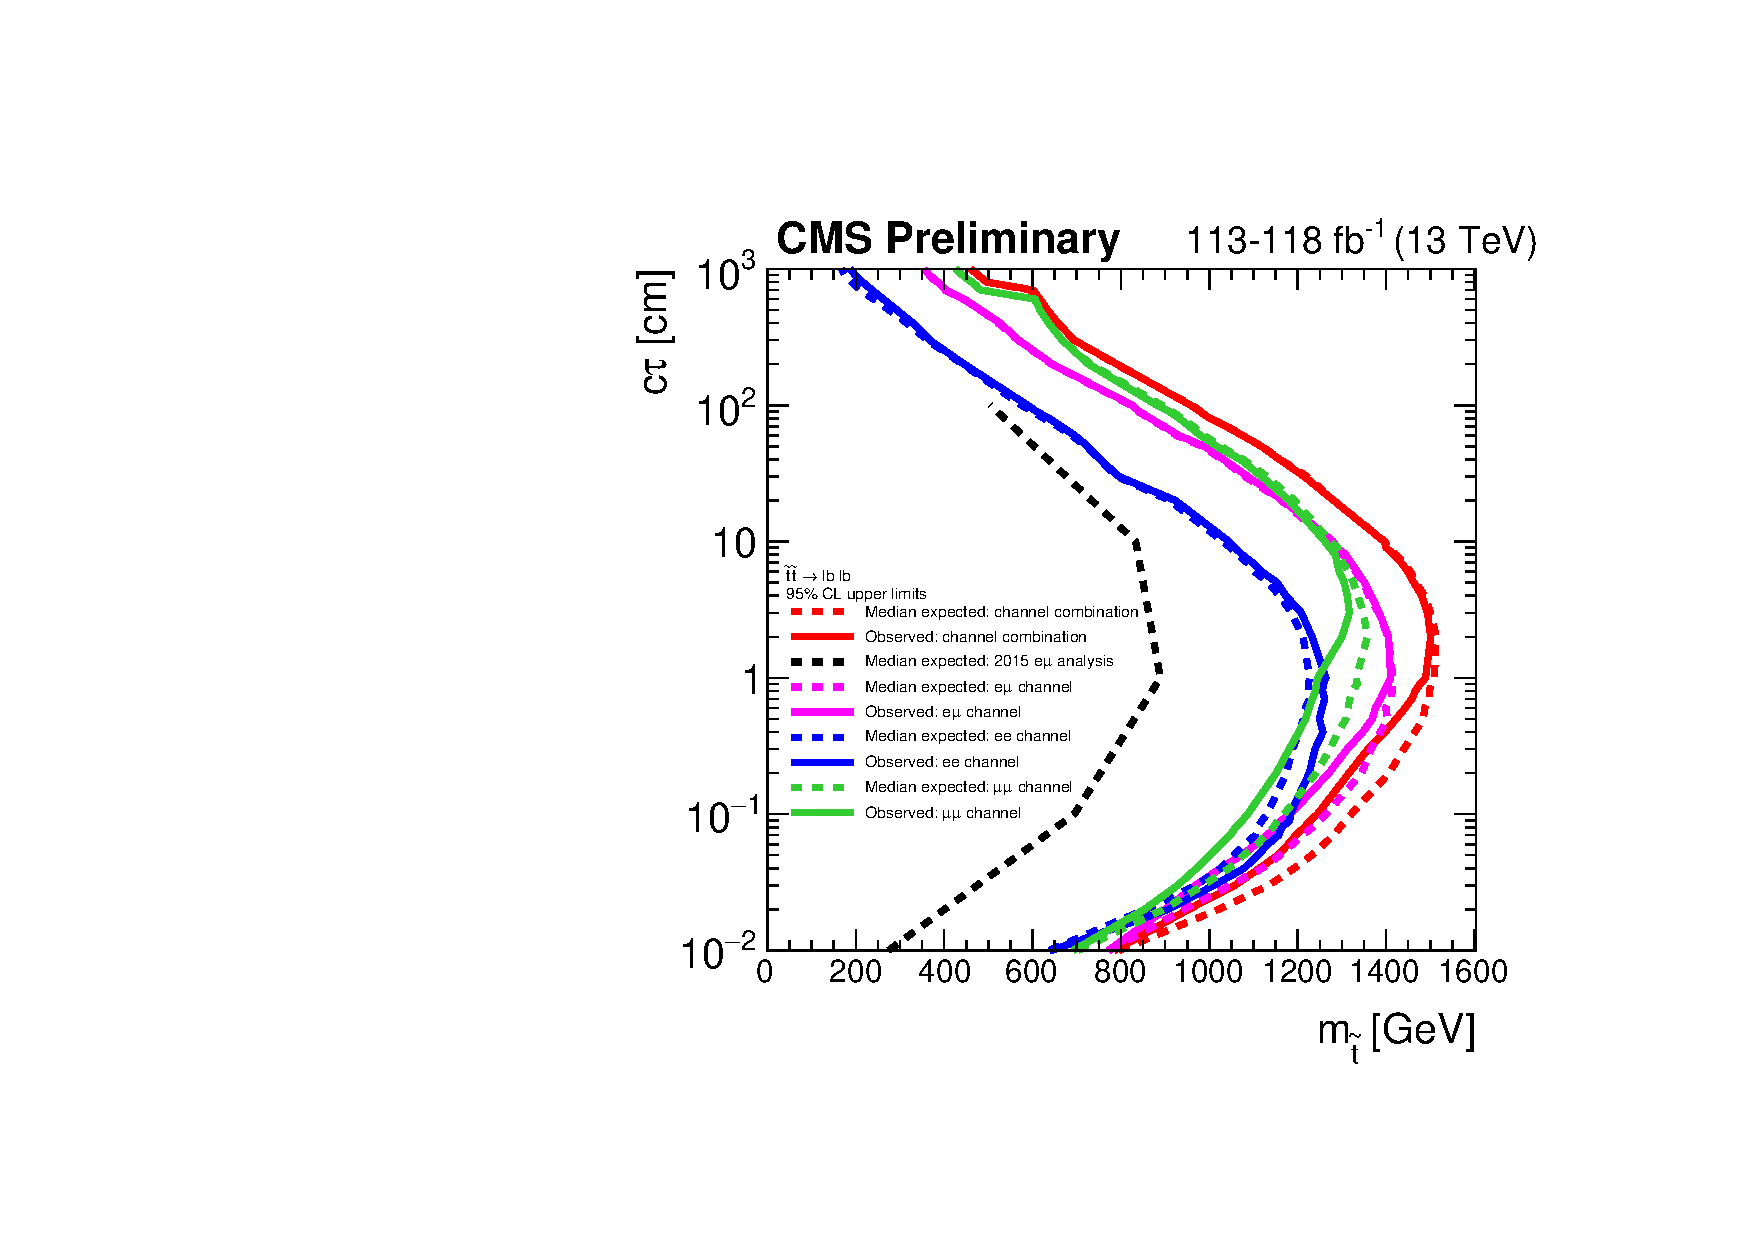
\includegraphics[width=0.65\textwidth]{figures/results/2DlimitsStopToLB.pdf}
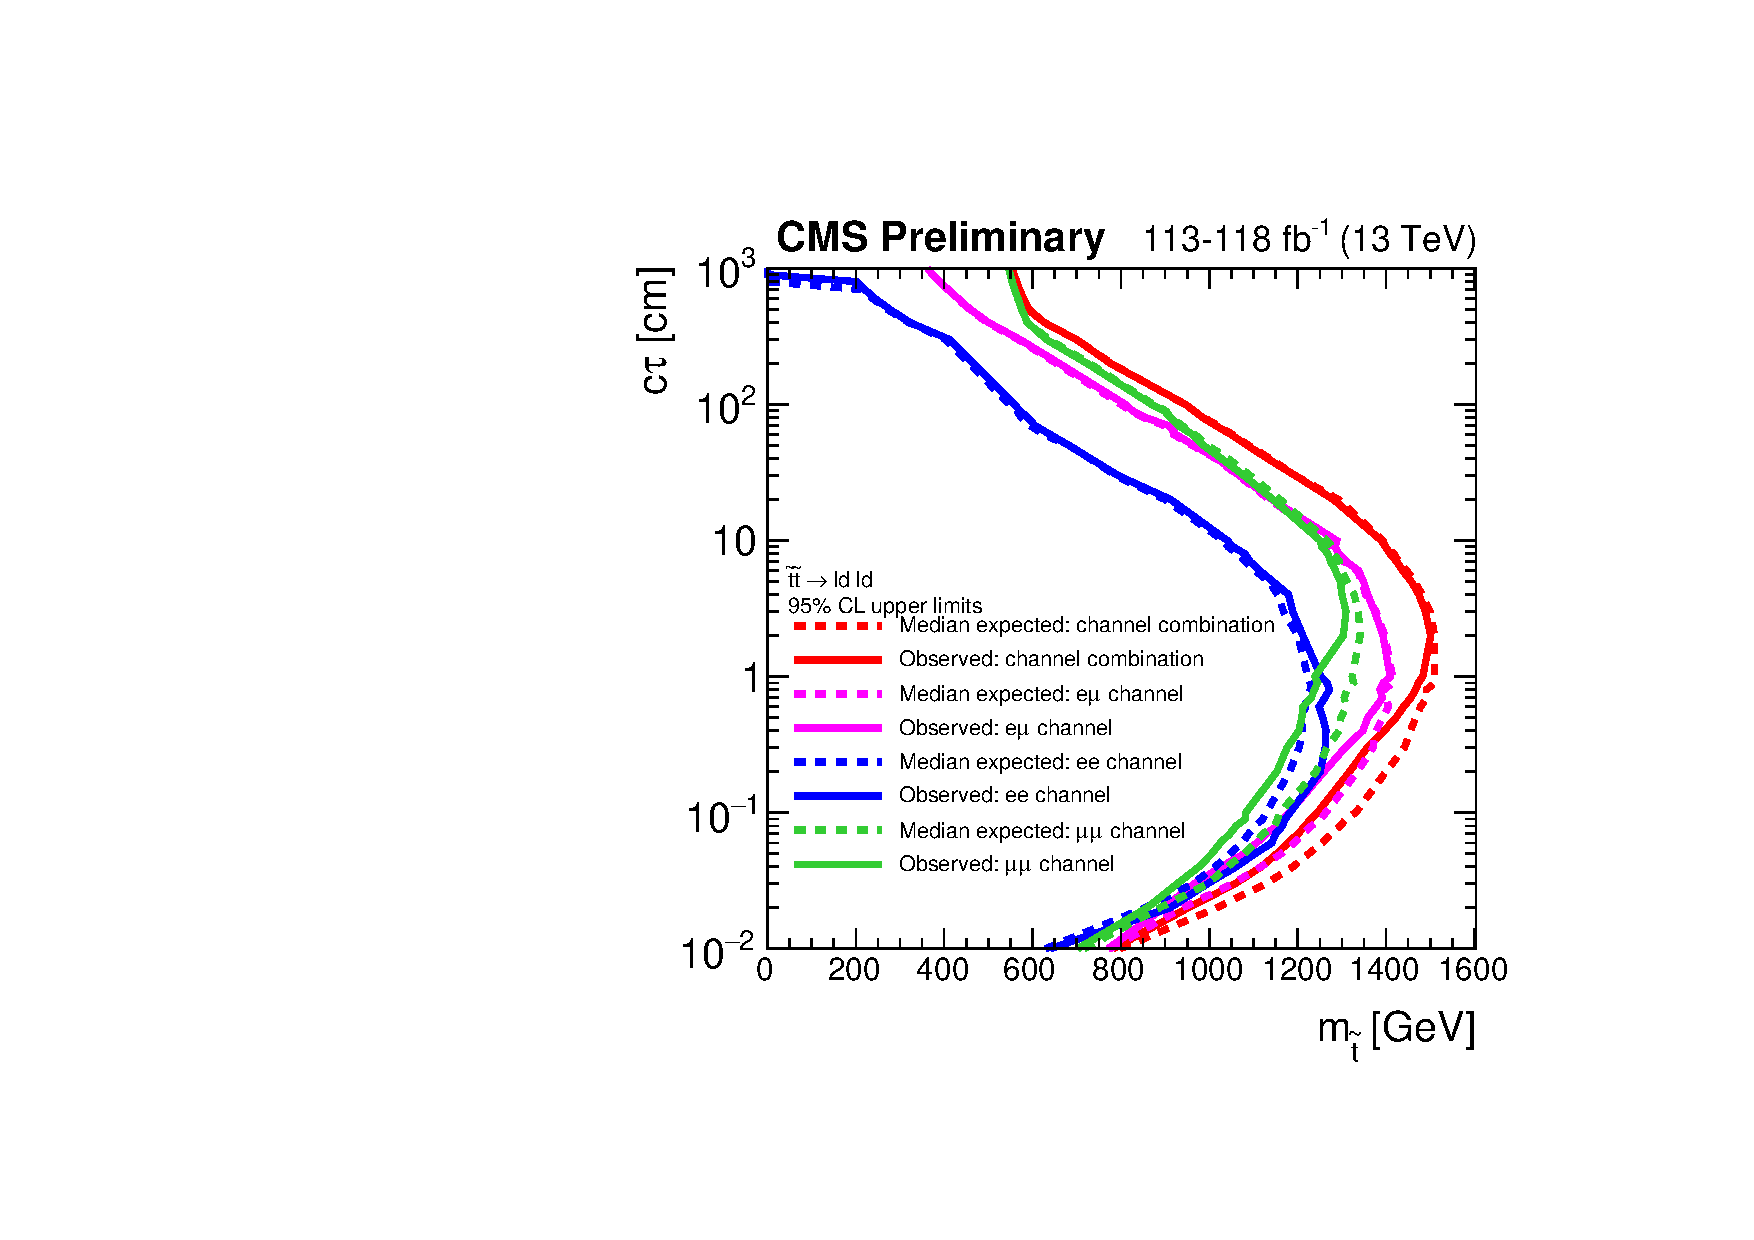
\includegraphics[width=0.65\textwidth]{figures/results/2DlimitsStopToLD.pdf}
\caption{The 95\% $\CL$ upper limits on the long-lived particle mass ($m_{\PSQt}$) as a function of its lifetime ($c\tau$), for the $\Pe\Pgm$, $\Pe\Pe$, and $\Pgm\Pgm$ channels. The \stoptolb (top) and \stoptold (bottom) processes are shown.} 
%The $\PSQt\PASQt \to \PAl\PQb\:\Pl\PAQb $ (upper left), $\PSQt\PASQt \to \PAl\PQd\:\Pl\PAQd$ (upper right), $\PSl\PASl \to \PAl\PXXSG\:\Pl\PXXSG$ (lower left), and $\PH \to \PS\PS \to \Pl\PAl\:\Pl\PAl$ (lower right) processes are shown.}
\label{limits_individual}
\end{figure}

\begin{figure}
\centering
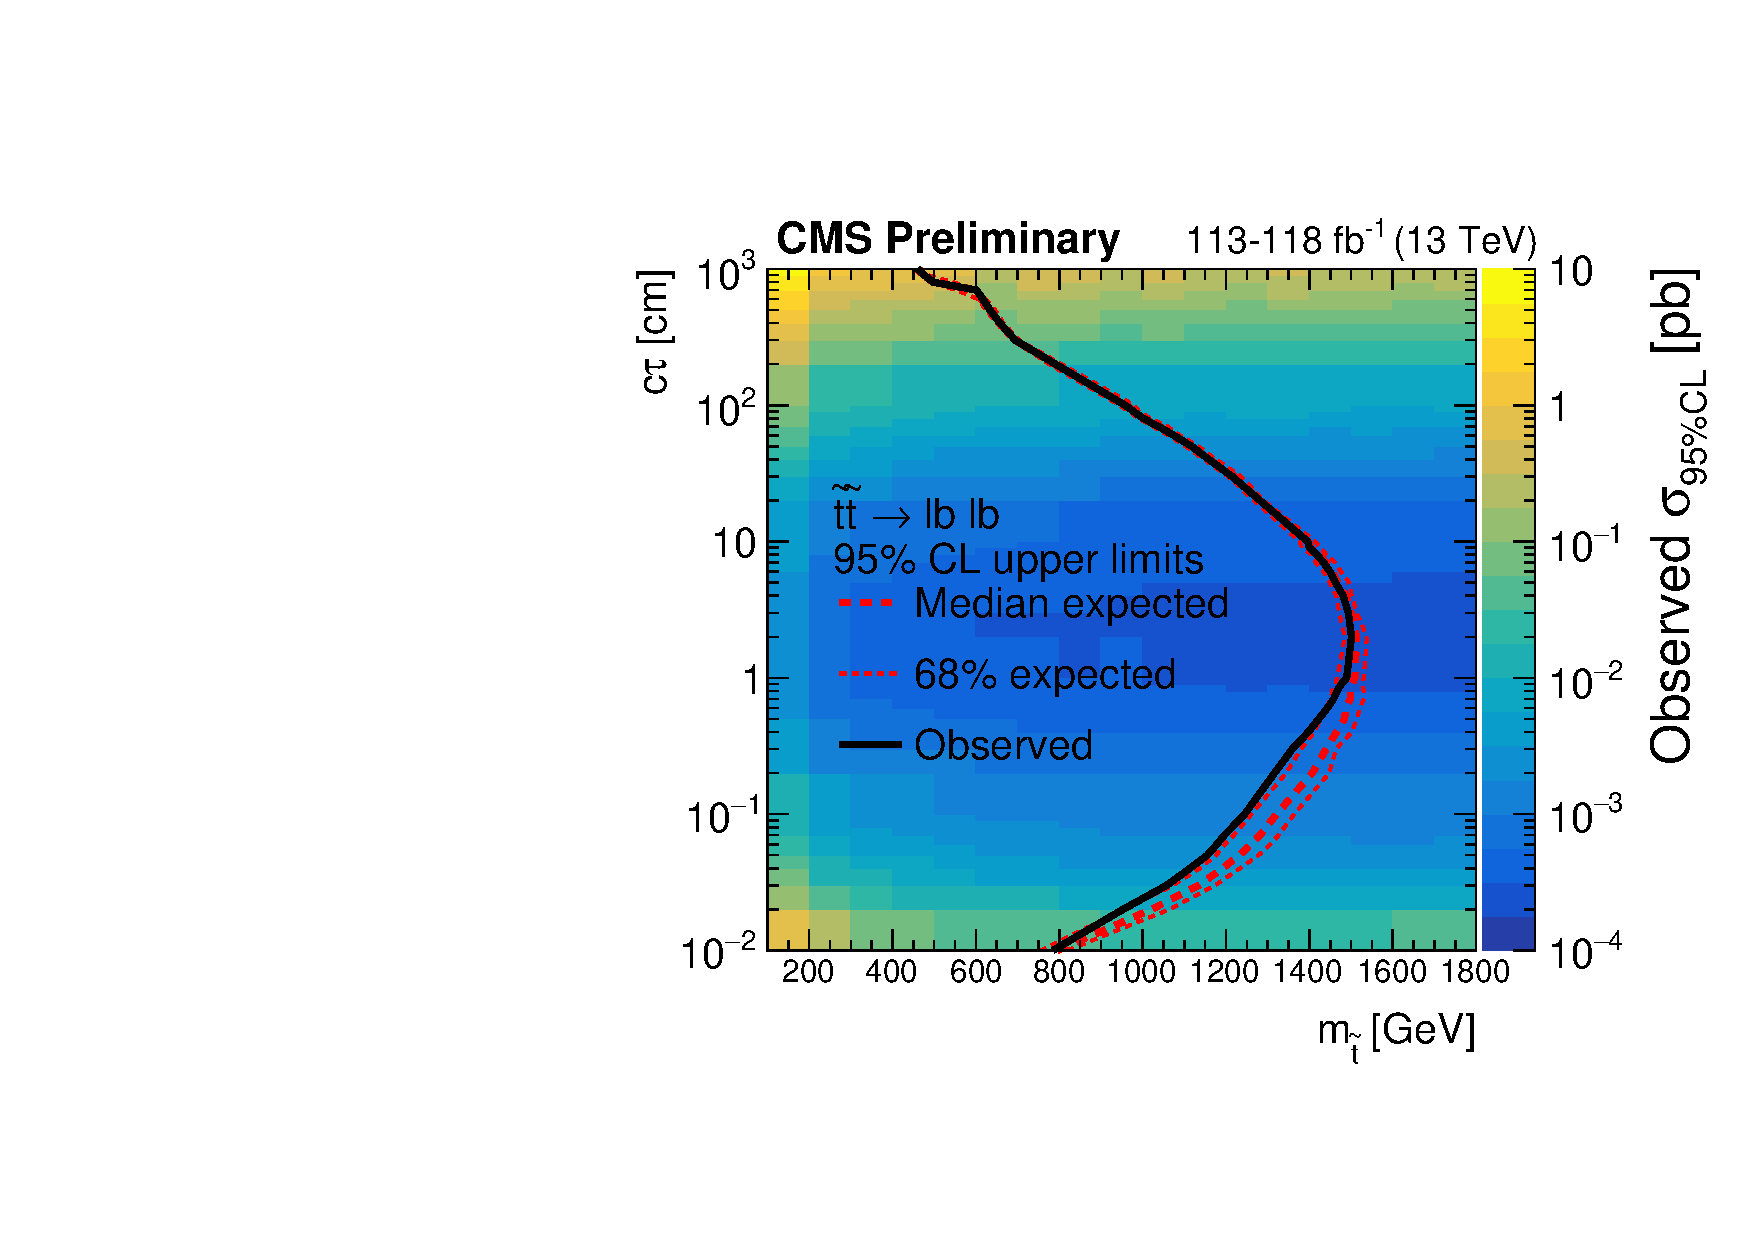
\includegraphics[width=0.65\textwidth]{figures/results/2DlimitsCombinedStopToLB.pdf}
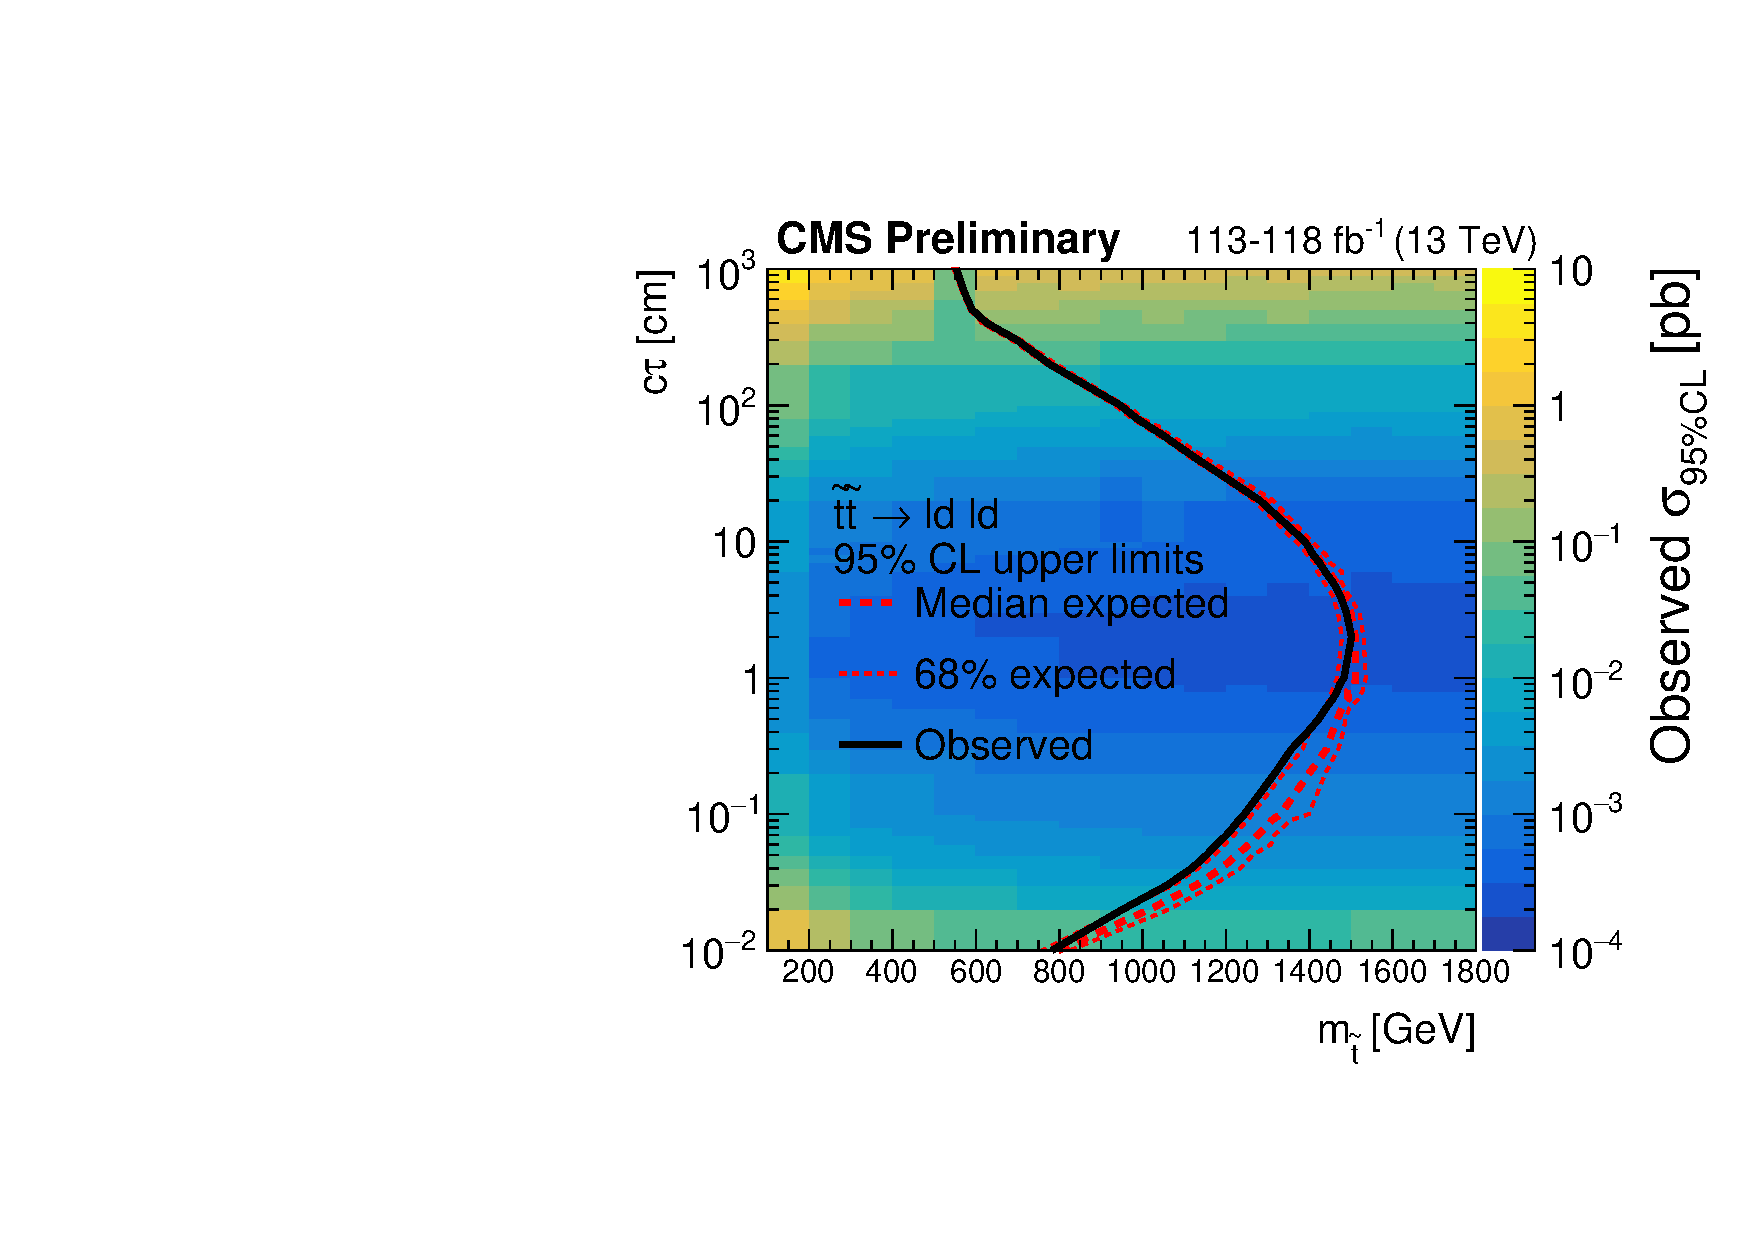
\includegraphics[width=0.65\textwidth]{figures/results/2DlimitsCombinedStopToLD.pdf}
\caption{The 95\% $\CL$ upper limits on the long-lived particle mass ($m_{\PSQt}$) as a function of its lifetime ($c\tau$). The colors indicate the observed 95\% $\CL$ upper limit on the cross section. The \stoptolb (left) and \stoptold (right) processes are shown.} 
%The $\PSQt\PASQt \to \PAl\PQb\:\Pl\PAQb $ (upper left), $\PSQt\PASQt \to \PAl\PQd\:\Pl\PAQd$ (upper right), $\PSl\PASl \to \PAl\PXXSG\:\Pl\PXXSG$ (lower left), and $\PH \to \PS\PS \to \Pl\PAl\:\Pl\PAl$ (lower right) processes are shown.}
\label{limits_combined}
\end{figure}